\section{Minimax Algorithm} 
\label{sec:Minimax Algorithm}

\subsection{Introduction to Minimax}
\label{subsec:Introduction to Minimax}
The Minimax algorithm is a recursive algorithm which is used in turn-based games like chess and tic-tac-toe, 
to make the AI player consider all possible moves and choose the most rational one.

\subsection{Explanation of Minimax}
\label{subsec:Explanation of Minimax}
\subsubsection{About Minimax}
First, it is important to understand the meaning behind recursive code. 
When code is recursive, it for example means that it's a function that calls itself with updated arguments until it reaches some condition the function wants to return. 
In the Minimax algorithm, the function is made to call itself in order to keep looking at more possible future moves, 
and ultimately decides which move is the best move to make on the AI’s current board.
\subsubsection{Why is it called Minimax}
The idea behind minimax is that the algorithm expects the game to be a turn-based 2-player game, and the algorithm defines these 2 players as the minimizer and the maximizer. 
This simply means that the algorithm always expects the minimizer to pick the move with the lowest score, and the maximizer to do the opposite. 
Here is an example: Here the maximizer is the human player and the minimizer is the AI player in this scenario.\\
\begin{figure}
    \caption{An example of a Tic-Tac-Toe board. [\ref{bib:Tic-Tac-ToeBoard}]}
    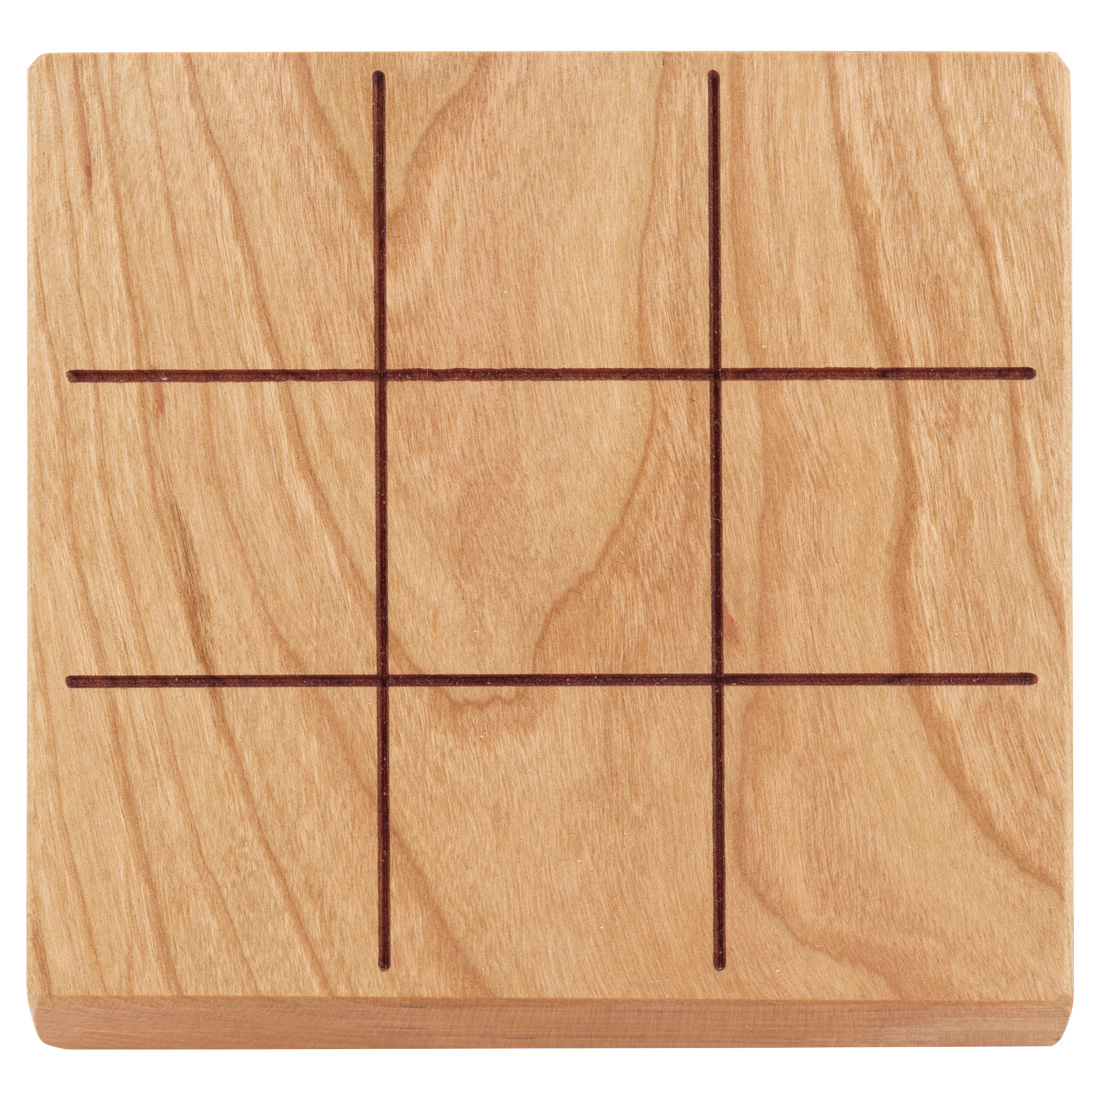
\includegraphics[width=\textwidth]{89-137-4480.jpg}
    \label{fig:Board Example}
\end{figure}\\
Consider the Tic-Tac-Toe board in figure~\ref{fig:Board Example}.\\\\
In this scenario the AI player goes first as “X” and tries to figure out the most rational move of the 9 moves possible. 
It does this by predicting what the opposing player, maximizer would then do on his next move and so on until it has found the fastest way to win for that one move. 
Basically, the algorithm runs a simulated game on each of the current board’s possible moves, against the maximizer, 
and when it is done with one move it backtracks back to the current board with that moves score value, to run a new simulation on the next move. 
When it has simulated how to win by all the possible moves it will then make the move that will help it win the fastest.\\\\
Consider again another example in figure~\ref{fig:Tree Example}.\\
\begin{figure}
    \caption{Minimax Tree Example. [\ref{bib:MinimaxTreeExample}]}
    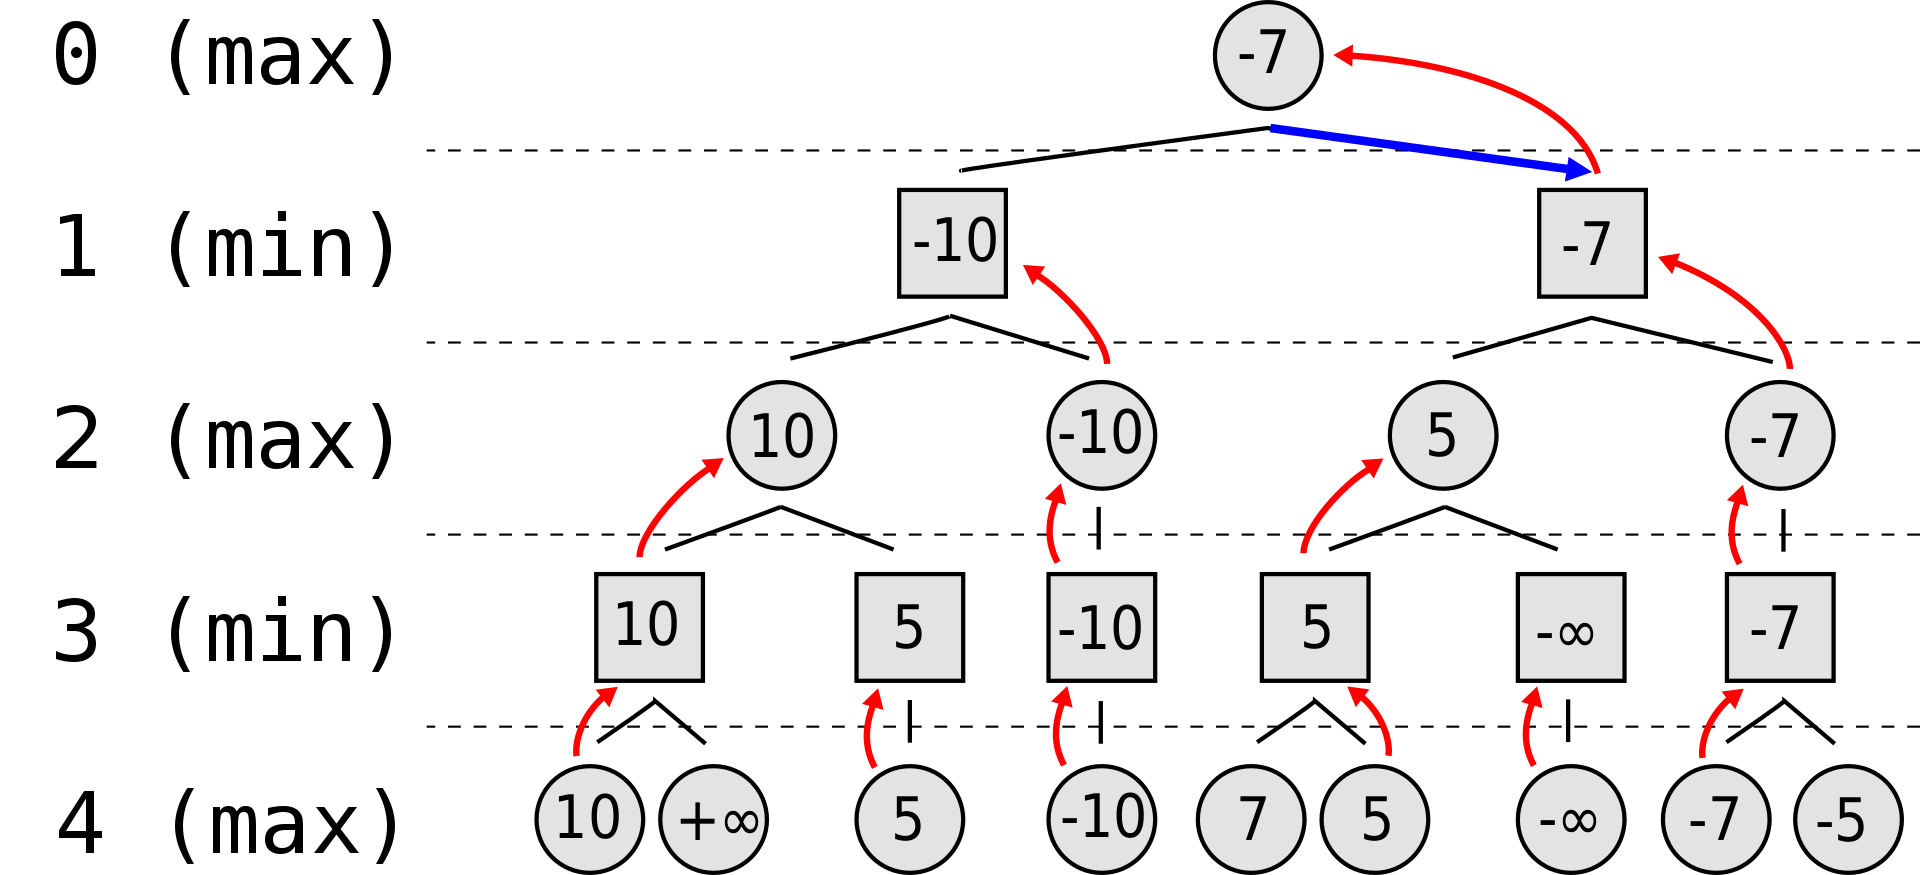
\includegraphics[width=\textwidth]{1920px-Minimax.svg.png}
    \label{fig:Tree Example}
\end{figure}\\
The Minimax tree shows an example of how the minimax works. In this scenario the maximizer goes first, and has 2 possible moves. 
The maximizer would therefore explore the first move first, marked -10. At this point the algorithm has not simulated this move yet and therefore does not know that value yet. 
So first it just tries the moves leftmost in the tree until it hits the depth 4 which is the bottom in this scenario. It would end up with a value of 10 which would be good for the maximizer. 
However, the minimizer needs to be taken into account, so the maximizer backtracks once to see the other move which is +infinity. 
It is guaranteed, that the minimizer would never pick that route, which means the score 10 can be kept in mind while the maximizer backtracks to the next point where the minimizer has a move. 
As is seen this route only gives both players one choice on each of their respective turns. 
The last move has a -10 score so it backtracks with that score once again and ends up with 10 and -10 on the 2 moves the minimizer can make. 
If the maximizer chooses this route the point value of the move would therefore be -10 as the minimizer always goes for the lesser score.\\
The algorithm then does the same thing for the other branch of moves and finds that this move will serve the maximizer better as it will yield -7 move value which is still poor for the maximizer but less so than a -10 score.\\\\
The explanation written here is based on \href{https://www.youtube.com/watch?v=l-hh51ncgDI}{this video from 0:00 to 2:30}.[\ref{bib:MinimaxVideo}]
\clearpage
\subsection{Implementation of Minimax}
\label{subsec:Implementation of Minimax}
% Show our own code!
\begin{lstlisting}[language=python, caption={python example}, label={Script}, basicstyle=\ttfamily\small]
    # AI makes a move based on minmax algorithmic search for the most rational move to make
    def ai_move(board):
        best_move = board
        best_value = float('-inf')
        for move in all_possible_moves(board, AI):
            #print(move)
            move_val = minimax(move, 0, False)
            #print(move_val)
            if move_val > best_value or best_value == None:
                best_move = move
                best_value = move_val
        return best_move
\end{lstlisting}
The function ai\textunderscore move gets called when its the AI's turn to play. The function generates a list of all possible moves from the current board, 
which the function recieves from the arguments.
This list is then iterated over to run the minimax recursion on each of these possible moves.
When the result move\textunderscore val is received for the current move, this value is then checked to see if it is higher or equal to the stored best\textunderscore value. 
If it is, that stored value is then overridden with the new best value.
\begin{lstlisting}[language=python, caption={python example}, label={Script}, basicstyle=\ttfamily\small]
    def minimax(board, depth, isMax):
    score = evaluate(board)
    
    if score == 10: 
        return score
    if score == -10:
        return score
    if board.count(EMPTY) == 0:
        return 0

    if isMax:
        best = float('-inf')
        for move in all_possible_moves(board, AI):
            best = max(best, minimax(move, depth + 1, not isMax))
        return best
    else:
        best = float('inf')
        for move in all_possible_moves(board, HUMAN):
            best = min(best, minimax(move, depth + 1, not isMax))
        return best
\end{lstlisting}
This is the implementation made in the Original Jupyter Notebook. 
The function always starts by checking the board with another function called evaluate. 
This function checks for win conditions and returns either 10 if the AI has a winning board and likewise -10 for the Human player.
If no one has won yet it returns 0.\\
Next the received score is checked to find out if the recursion for this move should end. This is done if the score is -10, 10 or 0, 
and as expected the move will not be considered as best 
if the score is -10 as the AI does not want the human player to win.\\
The next part of the implementation is the interesting part. First the current simulated move is checked to see if it is the maximizer's (Human) or the minimizer's (AI) turn. 
Depending on the result of this the recursion is set up oppositely. A "best" variable is started at the worst value for the player being 
-infinity for the maximizer and infinity for the minimizer. This is done to ensure that there is a value to overwrite on the very first run of the algorithm.
A list of possible moves is then created for this current simulated board and iterated over. This is where the recursion happens.
The minimax function is called within it self on the current considered move of the list. This ensures that all possible moves are evaluated for this new current board as well, 
because every time the function returns "best" it backtracks to check the next move. Remember the tree example explained in figure~\ref{fig:Tree Example}.\\\\
The implementation described here is based on the pseudo code explained in \href{https://www.youtube.com/watch?v=l-hh51ncgDI}{this video} from 2:30 to 5:20.[\ref{bib:MinimaxVideo}]
\clearpage